\chapter{Introducing the Jazz Trio Database}\label{chap:jtd_tismir}

\section{Introduction}

Given its lack of notated scores and the freedoms afforded to its performers, improvised jazz is a musical genre that has often resisted computational analysis. Recent advances in automatic music transcription, however, have enabled the creation of several large-scale databases of annotated jazz recordings \citep[e.g.,][]{Edwards2023, Foster2021}. This allows researchers to scale up the analysis of jazz improvisation to a degree that has not previously been possible.

Previous research has tended to focus on individual soloists and the annotation of accompanying musicians has tended to be incomplete or partial (only some members of the ensemble, for instance). Our goal in this project was to develop a database that included annotations for every musician in an improvising jazz ensemble. We focussed primarily on timing, as this enables the analysis of interesting group-level musical features, such as interaction and synchronization. However, we also wished to include automatically extracted pitch and velocity data for instruments where this has seen some previous work \citep[e.g., piano: see][]{Kong2021}.
		
To extract data from a mixed ensemble recording, we leveraged recent developments in audio source separation and timing annotation. Using deep learning, it has become possible to separate isolated sources from an audio mixture with massively increased fidelity compared to earlier approaches. The quality of separation still depends on the instrument, however, with vocals, bass, piano, and drums separation having seen the majority of work, while the separation of brass and stringed instruments remains at an earlier stage.
		
To this end, in this chapter we introduce the Jazz Trio Database (\GLS{JTD}), a database of machine-annotated recordings of piano soloists improvising with bass and drums accompaniment. These instruments form the standard ``rhythm section'' that has accompanied soloists in jazz since the 1940s, and can be thought of as providing the crucial contexts within which their improvisations are articulated and developed. To this extent, results obtained from our database could readily be generalized beyond the piano trio.

We identified recordings for inclusion in \GLS{JTD} by scraping user-based listening and discographic data and pulling audio from YouTube. We then used source separation models to extract isolated audio from each instrument, and finally applied a range of automatic transcription algorithms to automatically generate annotations from each source.
		
In this chapter, we describe several related datasets, discuss the curation of JTD, outline the data extraction pipeline we developed, and explore \GLS{JTD} by conducting several analyses. We envisage that \GLS{JTD} will be useful in a variety of \GLS{MIR} tasks, such as artist identification and expressive performance modeling.

\section{Related Work}

\begin{sidewaystable}[t!]
\centering
\caption[Comparison of existing datasets for each instrument in the jazz piano trio.]{Comparison of existing datasets for each instrument in the jazz piano trio. *Note that RWC-Jazz has not been made available free and open source, meaning that it is not possible to provide full detail here.}
\label{tab:jtd_existing_datasets}
\begin{tabular}{l c c c c c c}
\toprule
\textbf{Instrument} & \textbf{Name} & \textbf{Method} & \textbf{Tracks} & \textbf{Duration (s)} & \textbf{Annotations} & \textbf{Metadata} \\
\midrule
\textbf{Piano} & \GLS{WJD} & Manual & 6 & 582 & 3,149 onsets & Beat, chord, section \\
 & \GLS{PiJAMA} & Automatic & 2,777 & 804,960 & 7,108,460 MIDI notes & N/A \\
 & RWC-Jazz & Manual & 5 & 1,672 & N/A* & Beat, section \\
 & \GLS{JTD} (ours) & Automatic & 1,294 & 159,668 & 866,116 onsets, 2,174,833 MIDI notes & Beat \\
\textbf{Bass} & \GLS{WJD} & Automatic & 426 & 49,010 & 5,000 beat-wise pitches & Beat, chord, section \\
 & FiloBass & Automatic + manual & 48 & 17,880 & 53,646 MIDI notes & Downbeat, chord \\
 & RWC-Jazz & Manual & 5 & 1,672 & N/A* & Beat, section \\
 & \GLS{JTD} (ours) & Automatic & 1,294 & 159,668 & 543,693 onsets & Beat \\
\textbf{Drums} & \GLS{WJD} & Automatic + manual & 67 & 6,506 & 28,851 cymbal onsets & Beat, chord, section \\
 & RWC-Jazz & Manual & 5 & 1,672 & N/A* & Beat, section \\
 & \GLS{JTD} (ours) & Automatic & 1,294 & 159,668 & 796,604 onsets & Beat \\
\bottomrule
\end{tabular}
\end{sidewaystable}

A summary of related datasets is given in Table \ref{tab:jtd_existing_datasets}.\clearpage

\subsection{Weimar Jazz Database}

The Weimar Jazz Database (\GLS{WJD}) contains note-for-note transcriptions of 456 improvised jazz solos \citep{Pfleiderer2017}. The note-level (pitches, onsets, offsets, intonation, and dynamics) annotations are aligned to the original audio, and the database also includes annotations of chord sequences, beat, and measure numbers. In the initial release of the database, the majority of the annotations were created manually: only dynamics and intonation were measured automatically. 

Subsequent projects have extended the \GLS{WJD} to include automatic transcriptions of both the bass \citep{Abesser2017} and drum \citep{Dittmar2018} accompaniments. However, these are only partial annotations --- consisting respectively of beat-wise pitch transcriptions and the ``swing ratios'' played by the drummer on their ride cymbal --- which may limit their usability in future work.

\subsection{FiloSax and FiloBass}

The FiloSax dataset \citep{Foster2021} is a collection of 24 hours of annotated jazz performances by five tenor saxophonists, recorded against a pre-recorded backing of piano, bass, and drums for 48 ``standard'' jazz compositions. Note-level annotations were created automatically for each recording using an algorithm and through manual transcription. The location of sections and timestamps were also annotated, enabling (for instance) the relative timing of the soloist to the accompaniment to be estimated.

FiloBass \citep{Riley2023} expands Filosax with transcriptions of the bassist's performance on each backing track. A source separation model was first applied to isolate this from the audio mixture, and a commercial automatic transcription algorithm was used to generate MIDI from this signal. FiloBass represents an important effort to use recent developments in music source separation to facilitate downstream annotation, which we expand upon here by providing annotations for every member in an ensemble.

\subsection{PiJAMA}\label{sec:jtd_pijama_description}

Piano Jazz with MIDI Annotations (\GLS{PiJAMA}) consists of 200+ hours of solo jazz piano performances transcribed using a pitch-to-MIDI algorithm \citep{Edwards2023}. The methodology used by the \GLS{PiJAMA} authors has several similarities with our contribution: curated playlists of relevant music were developed by scraping discographic services and audio was downloaded from YouTube. Although comprehensive, \GLS{PiJAMA} only covers solo piano recordings, while the authors acknowledge that it is far more common for jazz pianists to perform in a trio with bass and drums.

\subsection{RWC-Jazz}

Five of the 50 recordings contained in the RWC-Jazz database \citep{Goto2002} feature a lineup of piano, bass, and drums, with a total duration of 28 minutes. To the best of our knowledge, this is the only database with complete annotations provided for every musician in a jazz ensemble. These annotations were created manually and consist of MIDI data for each instrument, alongside beat, downbeat, and section timestamps.

\section{Database Curation}

\begin{figure}[htbp]
  \centering
  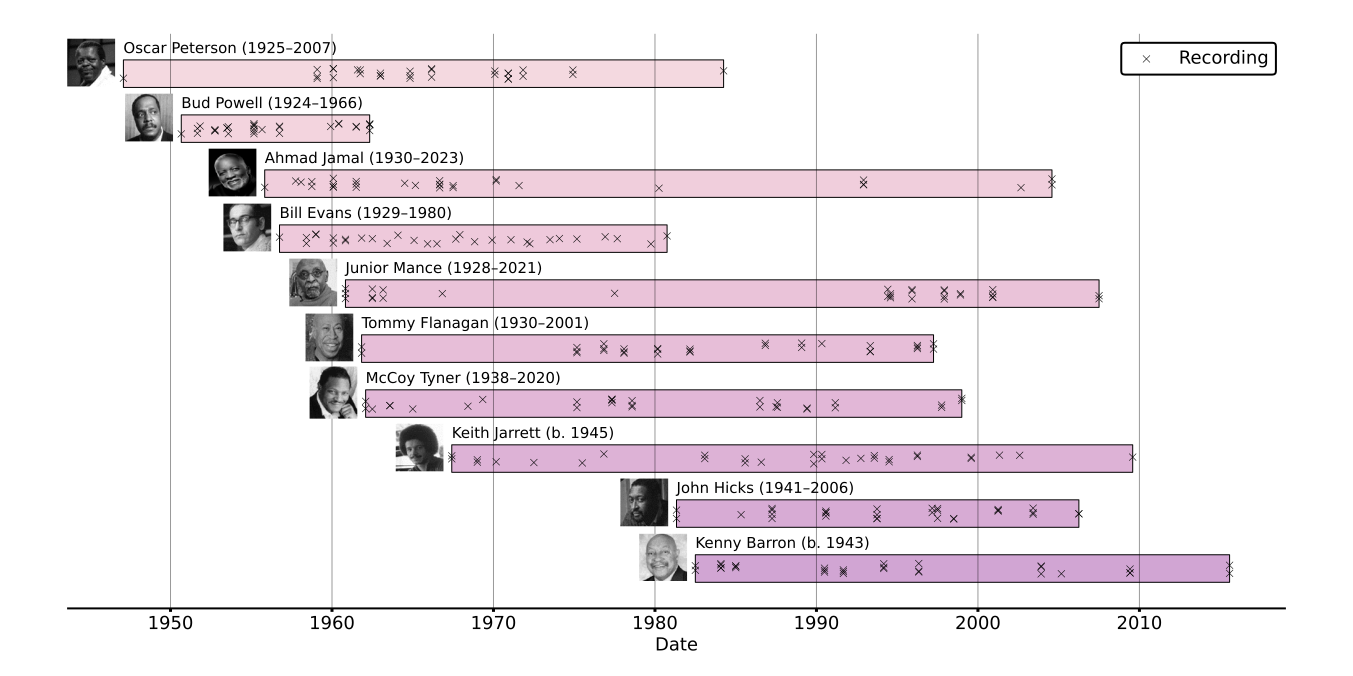
\includegraphics[width=0.9\textwidth]{figures/jtd/figure_1.png}
  \caption[Process followed for constructing JTD.]{Process followed for constructing JTD. Arrow block symbols indicate stages where tracks/artists may be removed.}
\label{fig:jtd_construction}
\end{figure}

When compiling any database of music recordings, deciding which material to include can be challenging. To simplify the process, we first identified a body of suitable ensembles, and then identified appropriate recordings from their discography to include in JTD. Our database curation and annotation procedure is shown in Figure \ref{fig:jtd_construction}.

\subsection{Performer Selection}

The criteria used to decide whether an artist should be included in \GLS{JTD} was that they should be both ``popular'' and ``prolific''. With relation to ``popularity'', we wanted to ensure that artists would only be included if they were both representative of general jazz listening habits and were highly regarded by experts. With relation to ``prolificacy'', we wanted to ensure that artists would only be included if they had recorded a significant amount of material in the piano-bass-drums trio format.

\subsubsection{Identifying ``Popular'' Performers}

We searched the Last.fm platform to obtain an overview of jazz listening habits. Last.fm is an online recommendation service that allows users to build profiles of their personal taste by tracking the music they listen to across many streaming platforms. We scraped the names of the top 250,000 performers and groups on Last.fm most frequently tagged by users with the genre ``Jazz'', using their official API.\footnote{\url{https://www.last.fm/api}} We ordered by tag count, rather than by plays or favorites, as we wanted to find the most quintessentially ``jazz'' artists, rather than those who fused jazz with other styles. 

\begin{figure}[t!]
  \centering
  \includesvg[width=0.75\textwidth]{figures/jtd/figure_2}
  \caption[Total streams (``scrobbles'') of all recordings made by the top 20 ``trio'' artists most-frequently tagged as ``Jazz'' on Last.fm.]{Total streams (``scrobbles'') of all recordings made by the top 20 ``trio'' artists most-frequently tagged as ``Jazz'' on Last.fm.}
\label{fig:jtd_total_streams}
\end{figure}

From the resulting list of performers and groups, we selected only those with the word ``Trio'' in their name. This left 249 unique performers or groups. While the names of many of the ``usual suspects'' featured prominently in this list (e.g., Bill Evans, Keith Jarrett), it also included several performers that were mainly known in other genres (e.g., Dee Felice, who accompanied soul singer James Brown when he performed jazz standards) or that mostly composed soundtrack or ``stock'' music (e.g., Vince Guaraldi, famous for the soundtrack to ``A Charlie Brown Christmas'': see Figure \ref{fig:jtd_total_streams}).

We then cross-referenced the Last.fm results against two major jazz textbooks, keeping only those artists that received a mention in the discographies of either Ted Gioia's ``The History of Jazz'' \citeyearpar{Gioia2011} or Mark Levine's ``The Jazz Piano Book'' \citeyearpar{Levine2011}. The intention here was to capture artists regarded highly by jazz experts. We note, however, that the retrospective nature of these textbooks could have meant that performers who have become active only in recent years (or, indeed, in the time since their publication) were excluded; future revisions of \GLS{JTD} may use subsequent editions of both textbooks. 

This narrowed the total number of groups to 33, all of which were named after a single musician (e.g., the Oscar Peterson Trio). This musician would have led the ensemble and typically composed the majority of the compositions they would play. Two bandleaders were bassists (Dave Holland and Ray Brown) and the remainder were pianists; no bandleaders were drummers.

\subsubsection{Identifying ``Prolific'' Performers}

Next, we turned to searching the MusicBrainz service to acquire a more detailed summary of each bandleader's recorded discography. MusicBrainz is a community-driven service that provides a comprehensive and open index of discographical metadata (including artist names, recording locations, and release dates) and is commonly used in music information retrieval tasks. We scraped MusicBrainz using their API to gather metadata relating to every individual recording ever made by each of our 33 bandleaders.\footnote{\url{https://musicbrainz.org/doc/MusicBrainz_API}} This resulted in the identification of 18,504 recordings.

We removed recordings that (1) were duplicated across several releases (for instance, those that also appeared on compilation albums), (2) did not contain a complete trio lineup, or that included multiple musicians performing on one instrument (for example, a piano ``four hands'' recording), (3) featured a musician doubling on a second instrument (for instance, a pianist who also played synthesizer, or a drummer who played auxiliary percussion), and (4) contained keywords in their title that suggested that they were incomplete performances (e.g., ``breakdown'', ``outtake'', ``false start'').

Four of the 33 bandleaders recorded less than an hour of material in the trio setting; amongst these, Dave Brubeck, Count Basie and Joe Zawinul were all better known for their work leading larger ensembles, while Art Tatum worked mainly in a trio of piano, bass, and guitar. After omitting the recordings by these bandleaders, 4,659 tracks remained.

\subsection{Recording Selection}

\subsubsection{Inclusion Criteria}\label{sec:jtd_inclusion_criteria}

To obtain a consistent set of tracks that could be analyzed reliably by our automated pipeline, we defined inclusion criteria to compare each recording against before including it in JTD. A track must have had: (1) an approximate tempo between 100 and 300 quarter-note beats-per-minute (BPM), assessed by tapping along to the opening measures of the performance, (2) a clear quarter note pulse, with a time signature of either three or four beats per measure (and with no changes in meter), (3) an identifiable piano solo, accompanied by bass and drums with no interruptions in the ensemble texture (i.e., ``solo breaks''), (4) an uninterrupted ``swing eighths'' rhythmic feel, and (5) a link to the recording on YouTube.

Additional criteria were specified for each instrument in the trio. During their solo, pianists must have played on acoustic instruments (rather than, e.g., synthesizer or ``Rhodes'' piano), and without any external FX (e.g., reverb, distortion). Bassists must also have played on an unmanipulated acoustic instrument using their fingers or a plectrum, not a bow. Drummers must have used a traditional ``traps'' kit (snare and kick drums; multiple cymbals, including hi-hat, ride, and crash; tom-toms), without auxiliary percussion (e.g., shakers, maracas). This must also have been played using sticks, rather than wire brushes or cloth mallets. 

These requirements were included so as to (1) ensure that all notes had clear onset times, and (2) maximize the acoustic similarity between the recordings in the dataset and the distribution of (pop, rock) material typically used to train audio source separation models. 

\subsubsection{Metadata Curation}\label{sec:jtd_metadata_curation}

For the recordings that met the inclusion criteria, we combined the metadata scraped from MusicBrainz with additional fields compiled manually, including timestamps for the beginning and ending of the piano solo, the position of individual instrument sources across the stereo spectrum, and the time signature. YouTube URLs were scraped from the ListenBrainz service using the track identifiers returned from MusicBrainz and manually corrected in the case of any false positives. Audio was downloaded from the URLs, trimmed to the piano solo, and stored in a lossless format with a sample rate of 44.1 kHz.

We elected only to include audio from piano solos as this is typically the only section in a performance where every musician would be expected to improvise. For instance, in the ``head'' (melodic statements that occur at the beginning and ending of ``straight ahead'' jazz performances), the material is pre-composed; while, in bass or drum solos, the accompanying musicians may choose not to play \citep{Monson1996}.

\begin{figure}[t!]
  \centering
  \includesvg[width=0.75\textwidth]{figures/jtd/figure_3}
  \caption[Duration of piano solo excerpts by all bandleaders.]{Duration of piano solo excerpts by all bandleaders. Bar colour indicates subset (either \GLS{JTD} or JTD-300).}
\label{fig:jtd_solo_durations}
\end{figure}

Of the 4,659 recordings that were evaluated, 1,294 (27.8\%) were included in JTD. The combined duration of all piano solos in these recordings was 44.5 hours (Figure \ref{fig:jtd_solo_durations}). These recordings were made between 1947 and 2015, with a median recording year of 1972. The vast majority (93\%) had a time signature of four beats per measure.

\begin{figure}[t!]
  \centering
  \includesvg[width=0.75\textwidth]{figures/jtd/figure_4}
  \caption[Number of tracks featuring the 10 performers on each instrument with the most recordings in \GLS{JTD}.]{Number of tracks featuring the 10 performers on each instrument with the most recordings in \GLS{JTD}.}
\label{fig:jtd_tracks_by_performer}
\end{figure}

The recordings in \GLS{JTD} featured 34 different pianists, 98 bassists, and 106 drummers. Bassist Ray Brown and drummer Ed Thigpen performed together as a rhythm section on the largest number of individual recordings (94). Of those who were not also the leader of their own trio, bassists Ron Carter and Sam Jones accompanied the largest number of different pianists (7), while drummer Roy Haynes accompanied 6 pianists. Figure \ref{fig:jtd_tracks_by_performer} shows the number of tracks by the ten performers on each instrument with the greatest number of recordings in JTD.

\subsubsection{JTD-Brushes}

Excluding recordings where the drummer used wire brushes resulted in the removal of 973 tracks scraped from MusicBrainz. To address this imbalance, we created a separate set of annotations for tracks that were only rejected from \GLS{JTD} because of the use of brushes. We define this related database as JTD-Brushes. Note that the recordings in JTD-Brushes were not curated to the same extent as those in JTD; the full recording was used, rather than only the piano solo, and the time signature was estimated by the beat tracker automatically, rather than being provided beforehand. The duration of the recordings in JTD-Brushes was 79 hours. While the remainder of this article focuses on the curated JTD, we envisage that JTD-Brushes may be of use in developing or evaluating e.g., beat tracking or ``soft'' onset detection models \citep[e.g., ][]{Tomczak2023} that can cope with a broader variety of drumming techniques.

\subsection{Class Imbalance}\label{sec:jtd_class_imbalance}

A side effect of our inclusion criteria was that bandleaders who worked most frequently in the acoustic ``swing'' style were overrepresented in the JTD. Conversely, those who worked across a variety of styles or who frequently incorporated electronic elements into their music had very few recordings that met the inclusion criteria. The three bandleaders with the most audio in the \GLS{JTD} were Bill Evans (5.5 hours), Keith Jarrett (4), and Oscar Peterson (3.5). Meanwhile, Abdullah Ibrahim, Brad Mehldau, and Dave Holland were each represented in the \GLS{JTD} by less than half an hour of audio.

This class imbalance could prove problematic were predictive models to be trained on the JTD. To that end, we created a subset of \GLS{JTD} (defined as JTD-300), that includes an equal number of recordings from the ten bandleaders with the most audio in JTD, sampled chronologically across the duration of their careers. Together, recordings led by these ten musicians --- all of whom were pianists --- made up 62.6\% of the total duration of audio in \GLS{JTD} (see Figure \ref{fig:jtd_solo_durations}).

For each of these bandleaders, we sorted their tracks in \GLS{JTD} chronologically by the date of recording. In cases where a full date could not be obtained from MusicBrainz, a track was estimated to have been made either midway through the month (in cases where both a month and year were given) or year (when only a year was given) it was recorded. In cases where multiple dates were given for one track (i.e., when an album was recorded over a period of time, without dates being assigned to individual tracks), we took the midpoint of these dates. If no dates were provided at all, the track was excluded from selection.

\begin{figure}[]
  \centering
  \includesvg[width=1.0\textwidth]{figures/rsos_rhythm/figure_1}
  \caption[Duration of the recording career for each of the ten pianists included in \GLS{JTD-300}]{Duration of the recording career for each of the ten pianists included in \GLS{JTD-300}. Markers indicate the date of recordings that appear in \GLS{JTD-300}, randomly jittered horizontally and vertically for visual clarity.}
\label{fig:rsos_jtd300}
\end{figure}

\begin{figure}[]
  \centering
  \includesvg[width=1.0\textwidth]{figures/rsos_rhythm/figure_s1}
  \caption[Durations of recordings in \GLS{JTD-300}.]{Durations of recordings in \GLS{JTD-300}. Each column shows the total duration of the recordings by every bandleader with recordings in \GLS{JTD-300}, with the green proportion corresponding with those tracks that are included within each subset (shown also as a percentage along the columns).}
\label{fig:rsos_bandleader_proportions}
\end{figure}

Next, we sorted each track into one of 30 equally spaced bins; the left edge of the first bin coincided with the date of a bandleader's earliest recording, and the right edge of the final bin with the day of their final (or most recent) recording. Tracks were ordered within each bin by the proximity of their recording date to the midpoint of that bin; if multiple recordings were made on the same day, they were arranged following the order in which they appeared on their original release. We then included the first track from each bin in JTD-300: in cases where a bin was empty, we added an additional track from the first bin, then the second bin, and so on, until 30 tracks were obtained for each bandleader (Figure \ref{fig:rsos_jtd300}). We show the proportion of recordings by each bandleader contained in JTD-300 within Figure \ref{fig:rsos_bandleader_proportions}.

\begin{figure}[t!]
  \centering
  \includesvg[width=0.75\textwidth]{figures/jtd/figure_5}
  \caption[Histogram grouping number of tracks in \GLS{JTD} by year of recording.]{Histogram grouping number of tracks in \GLS{JTD} by year of recording. Bar colour indicates subset (\GLS{JTD} or \GLS{JTD-300}.}
\label{fig:jtd_tracks_by_year}
\end{figure}

The combined duration of the audio in JTD-300 was 11.75 hours (26.4\% of the duration of JTD). As with JTD, these recordings were made between 1947 and 2015, with a median recording year of 1977.5. The distribution of recording years included in JTD-300 was comparable with \GLS{JTD} (Figure \ref{fig:jtd_tracks_by_year}). 95\% of JTD-300 recordings had a time signature of four beats per measure. We envisage that JTD-300 will most likely be of use in performer identification tasks or analyses of chronological trends in improvisation practice (here, see Chapter \ref{chap:rhythm_rsos}). Tasks that do not require balanced class sizes may be better accomplished using the full JTD.

\section{Annotation}

\subsection{Source Separation}

\subsubsection{Audio Channel Selection}

Before the development of full-spectrum stereophonic panning in the 1970s, audio signals could only be panned to the left or right speaker output, or both (center channel). For tracks in the \GLS{JTD} where at least one instrument in the trio was hard-panned in this manner (39\%), source separation was applied independently to the left and right monaural signals alongside the center output. The required channel was identified manually for each instrument during the metadata curation process (see section \ref{sec:jtd_metadata_curation}).

\subsubsection{Model Selection}

The \texttt{ZFTurbo} audio source separation model \citep{Solovyev2024} was used to separate each track in the \GLS{JTD} into four sources; ``bass'', ``drums'', ``vocals'', and ``other'' This model combines three existing source separation models and achieved the first prize in a recent community sound demixing competition \citep{Fabbro2024}. 

\subsubsection{Audio Preprocessing}\label{sec:jtd_audio_preprocessing}

As the \texttt{ZFTurbo} model was not trained explicitly to separate piano audio, we used the ``other'' source (consisting of the residual audio after removing every other source from the mixed signal) for this instrument. This meant it was possible that audio from the bass and drums could have ``bled'' into this track, which would have affected the performance of our downstream annotation pipeline.

To mitigate this possibility, prior to annotation we filtered the ``other'' source using a second-order Butterworth bandpass filter. Our goal was to attenuate frequency bands that could also be occupied by the drums and bass, while minimizing any damage to the quality of the piano audio. The filter was set to attenuate frequencies outside the range of 55--3520 Hz, equivalent to a six-octave span from $A_1$--$A_7$: as shown in Edwards et al. \citeyearpar{Edwards2023}, the vast majority of note events in jazz piano performance typically fall within this range. 

We demonstrate in section \ref{sec:jtd_alternate_methods} that filtering the piano audio improved the accuracy of our onset annotation pipeline compared to using the raw audio, and that this particular frequency range performed better than an alternative, quantitatively ``narrower'' range.

\subsubsection{``Vocal'' Source}

Another possibility was that the unmixed ``vocal'' source could also contain piano audio, which would necessitate summing it with the ``other'' source. We manually inspected the ``vocal'' source across a sample of 34 recordings sampled from JTD-300 (see section \ref{sec:jtd_ground_truth_annotations}). In all of these cases, the ``vocal'' source was either silent or contained vocalizations of the musicians (or, occasionally in the case of a live recording, members of the audience) reacting to the performance. Therefore, the ``vocal'' source was not used for downstream data extraction.

\subsection{Data Extraction}

Our data extraction pipeline consisted of three components: (1) an onset detection algorithm, applied to each separated audio source (except ``vocal''), (2) a beat and downbeat tracking algorithm, applied to the raw audio mixture, and (3) an algorithm to match onsets with their nearest beat, in order to assign a metrical interpretation to each onset. Our implementations of (1) and (2) were from the \texttt{madmom} (version \texttt{0.17.0}) Python package \citep{Bock2016}. The default setting of 100 frames per second was used in \texttt{madmom}, such that near-simultaneous events with a time difference of less than one frame (likely including, e.g., piano chords) would be treated as a single onset.

\subsubsection{Onset Detection}\label{sec:jtd_onset_detection}

The \texttt{CNNOnsetDetector} function in \texttt{madmom} was used to detect onsets in the isolated audio obtained for each instrument in the trio. This algorithm came first in the most recent \texttt{MIREX} onset detection competition.\footnote{\url{https://nema.lis.illinois.edu/nema_out/mirex2018/results/aod/}\label{note:mirex_2018}} A convolutional neural network (\GLS{CNN}) is fed spectrogram frames of audio (at the default rate of 100 frames per second) to obtain an onset activation function; this envelope is then smoothed using a moving window and onsets are identified as local maxima higher than a predetermined threshold. Both the window size and the peak-picking thresholds were optimized separately for each instrument class in \GLS{JTD} (see section \ref{sec:jtd_validation_results}). In section \ref{sec:jtd_alternate_methods}, we demonstrate that, for detecting onsets in the \GLS{JTD} piano audio, this algorithm outperformed both an existing automatic piano transcription algorithm \citep{Kong2021} and a naive spectral flux approach.

\subsubsection{Beat Detection}\label{sec:jtd_beat_detection}

The \texttt{DBNDownBeatTracker} function in \texttt{madmom} was used to detect the position of quarter note beats and downbeats in the audio mixture. This algorithm came first in the most recent \texttt{MIREX} beat tracking competition.\footnote{\url{https://nema.lis.illinois.edu/nema_out/mirex2019/results/abt/smc/}} A recurrent neural network (\GLS{RNN}) is applied to frames from an audio spectrogram to distinguish between beats, downbeats, and non-beat classes; a dynamic Bayesian network (\GLS{DBN}) then infers meter from the RNN observations (using the default rate of 100 frames per second). Meter changes cannot be detected by this algorithm, which led us to incorporate this into our inclusion criteria (see section \ref{sec:jtd_inclusion_criteria}).\footnote{\citet{Foscarin2024} have since proposed an end-to-end algorithm that does not require \GLS{DBN} post-processing of an activation function, which alleviates constraints on meter while potentially leading to greater overall precision. This was not available at the time \GLS{JTD} was compiled, however.}

We applied this algorithm multiple times to a single track. First, the default parameters specified by the authors were used, with the tempo allowed to vary between 100 and 300 quarter note beats-per-minute (as specified in the inclusion criteria). This resulted in the timestamps changing tempo frequently, due to the lack of constraint in the parameter settings. 

To resolve this, we gradually reduced the range of permissible tempo values for the beat tracker over a number of iterations. First, we calculate the durations between successive beats as
\begin{align}
d_{i} = b_{i+1} - b_{i}, \ i = 1, 2, \dots, n-1, 
\end{align}
where $n$ is the total number of beats in the track. Then, we calculate the inter-quartile range of beat durations $IQR_d$ as
\begin{align}
IQR_d &= Q_3\left( \{d_1, d_2, \dots, d_{n-1}\} \right) - Q_1\left( \{d_1, d_2, \dots, d_{n-1}\} \right),
\end{align}
and use this to filter the initial durations $d$ where 
\begin{align}
d'_i &= \{ Q_1 - 1.5(IQR_d) \leq d_i \leq Q_3 + 1.5(IQR_d) \}, \ i = 1, 2, \dots, n-1.
\end{align}
Finally, we recalculate $Q_1$ and $Q_3$ using only values of $d'$ and set these as the new minimum and maximum tempo for the beat tracker in the next iteration of the process. The total number of iterations this process ran for was optimized for the recordings in \GLS{JTD} (see section \ref{sec:jtd_validation}).

The downbeat classes estimated from the RNN were then combined with the detected beat positions and the time signature for the recording in order to assign measure numbers to every detected timestamp. 

\subsubsection{Beat-Onset Matching}\label{sec:jtd_beat_onset_matching}

The final stage of our detection pipeline involved matching every beat with the nearest onset detected in each instrumental source. The size of the window used to match any given onset to the nearest beat varied depending on the tempo of a track. Onsets played up to one thirty-second note before and one sixteenth note after any given timestamp were included within the window; whichever onset had the smallest absolute distance to the beat was understood to mark the pulse. If no onsets were contained within a window, then the musician was considered to not have marked the pulse at that timestamp. 

Our rationale for using an asymmetric window came from previous research which has suggested that jazz soloists are more likely to ``lag behind'' and mark the beat later than their rhythm section, as opposed to earlier \citep{Butterfield2010}. Additionally, \citet{Corcoran2021} describe how notes played more than a thirty-second note earlier than a given beat act as a subdivision of the previous beat (i.e., a delayed, swung ``eighth'' note), as opposed to marking that beat itself. 

\subsection{Validation}\label{sec:jtd_validation}

\subsubsection{Ground Truth Annotations}\label{sec:jtd_ground_truth_annotations}

To evaluate the effectiveness of our annotation pipeline, we manually annotated beat, downbeat, and onset positions across a representative subsample of tracks. In particular, we wanted to check whether the pipeline was resilient to a range of possible recording qualities, and also to the styles of the musicians represented most prominently in JTD. Consequently, we adopted a systematic approach, annotating the earliest, middle, and final recordings made by each of the ten bandleaders in JTD-300. Owing to his overrepresentation in JTD, we also annotated an additional four tracks by Bill Evans (selected randomly from JTD-300) --- enough to ensure that the percentage of recordings led by Evans in the subsample (20.6\%) was equivalent to \GLS{JTD} (19.6\%).

Two of the authors and one research assistant created the reference annotation set. The annotations of the assistant were checked for consistency by the lead author. The combined duration of the 34 recordings in the subsample was 72 minutes. The median recording year was 1975, comparable with both \GLS{JTD} and JTD-300 (see sections \ref{sec:jtd_metadata_curation} and \ref{sec:jtd_class_imbalance}), and the range of recording years was identical (1947--2015). 88\% of recordings had a time signature of 4 quarter notes per measure. 

\subsubsection{Validation Results}\label{sec:jtd_validation_results}

The performance of the pipeline was determined by considering the proportion of detected annotations that occurred within a 50 ms window of a ground truth annotation. For every track in the subsample, separate precision, recall, and $F$-measures were computed for each class: (1--3) the onsets within each unmixed instrumental source, and (4) the quarter note beats and (5) downbeats within the audio mixture. When $F = 1.0$, every onset or beat detected by the pipeline could be matched with a ground truth annotation, with no onsets or beats unmatched. 

We applied the gradient-free, nonlinear optimization algorithm \texttt{subplex} \citep{Rowan1990} implemented in the \texttt{NLopt} (version \texttt{2.7.1}) Python package to set the parameters of the beat and onset detection algorithms separately for each audio source.\footnote{\url{https://github.com/stevengj/nlopt}} In every case, the mean value of $F$ across the entire hand-annotated subsample was treated as the objective function to maximize. Note that, for the beat detection algorithm, only the $F$-measure obtained from evaluating the beat timestamps --- not the downbeats --- was considered during optimization.

\begin{table}[h!]
\centering
\caption[Optimized results for onset detection per instrument]{Optimized results for onset detection per instrument, showing mean $F$-measure, precision, and recall. Brackets show \emph{SD}s.}
\label{tab:jtd_optimization_results}
\begin{tabular}{l c c c c c c}
\toprule
 & \textbf{Piano} & \textbf{Bass} & \textbf{Drums} & \textbf{Beats} & \textbf{Downbeats} \\
\midrule
\textbf{F-measure} & 0.93 (0.03) & 0.93 (0.05) & 0.95 (0.03) & 0.97 (0.05) & 0.63 (0.44) \\
\textbf{Precision} & 0.93 (0.04) & 0.94 (0.04) & 0.96 (0.04) & 0.97 (0.05) & 0.63 (0.44) \\
\textbf{Recall} & 0.93 (0.04) & 0.93 (0.07) & 0.94 (0.04) & 0.97 (0.05) & 0.63 (0.44) \\
\bottomrule
\end{tabular}
\end{table}

The values of $F$ obtained from the optimized parameter set are shown in Table \ref{tab:jtd_optimization_results}. The performance of the onset detection algorithm was broadly equivalent across instrument classes, with drums performing marginally better than bass and piano. In comparison with earlier results obtained from applying the same algorithm to equivalent multi-tracked audio datasets (``polyphonic pitched'', $mean(F) = 0.95$, ``plucked strings'', $mean(F) = 0.90$, ``solo drums'', $mean(F) = 0.93$, see note \ref{note:mirex_2018}), we obtained similar onset detection accuracy. This indicated to us that the source separation process was unlikely to have caused significant damage (in the form of artifacts, etc.) to the audio, to the point that onset detection algorithms trained on multi-tracked recordings could not also be applied to JTD.

While the beat tracking results indicated good performance, downbeat tracking was noticeably worse. To understand why, we inspected all tracks where $F(downbeat) = 0.0$, while $F(beat) > 0.95$ (i.e., the downbeats were out-of-phase). We observed that, in the majority of these cases, metrically ``strong'' beats were being mistaken for other ``strong'' beats (i.e., beat 2 and beat 4, in 4/4), rather than ``weak'' beats, and vice versa. This suggests that our results may still have some value in the analysis of metrical structure, and we also observed that our results were in line with those obtained from applying the same algorithm to other metrically complex forms of music.\footnote{\url{https://www.music-ir.org/mirex/wiki/2016:Audio_Downbeat_Estimation_Results}} However, future revisions of \GLS{JTD} may leverage the modular design of our codebase to integrate more sophisticated downbeat tracking algorithms \citep[e.g.,][]{Foscarin2024} as these become available.

Finally, we looked at the temporal difference between equivalent automatic and ground truth annotations. The pipeline tended to annotate beats and onsets earlier than the human annotators did; the mean difference in beat location time (algorithm--human) was $-4.82$ ms ($SD = 4.58$), and for onsets the mean difference was $-4.53$ ms ($SD = 3.42$). There were no substantial differences between onsets detected for different instrument classes here (piano, $-5.77$ ms, bass: $-4.29$ ms, drums: $-4.53$ ms). In context, this variation was likely perceptually sub-threshold, and should be negligible in most applications.

\subsubsection{Alternative Methods}\label{sec:jtd_alternate_methods}

Next, we compared several alternative onset detection methods, using the piano audio and corresponding ground truth annotations for evaluation. These methods were: (1) an automatic transcription model \citep{Kong2021}, which generates MIDI (incorporating both pitch and rhythmic information) from audio, (2) a naive audio signal processing approach, whereby onsets were identified as local maxima from a normalized spectral flux envelope, using the implementation from the \texttt{librosa} (version \texttt{0.8.1}) Python package \citep{McFee2015}, (3) the current approach, without the audio filtering described in section \ref{sec:jtd_audio_preprocessing}, and (4) the current approach, with a quantitatively ``narrower'' bandpass filter (attenuating frequencies outside the range of 110--1760 Hz i.e., $A_2$--$A_6$).

Note that, as method (1) generates multiple MIDI events for what would be regarded perceptually as a single onset (i.e., a chord), near-simultaneous MIDI events within a window of 50 ms were grouped together, with the onset of the earliest event taken as the onset of the whole group. The size of this window was optimized following the method described in \ref{sec:jtd_validation_results}, as were the individual parameter sets used to pick peaks from the activation functions returned separately from methods (2--4). The default setting of 100 frames per second was used for method (1).

\begin{table}[h!]
\caption[Onset detection results per method, piano only]{Onset detection results per method, piano only}
\label{tab:jtd_methods_comparison}
\centering
\begin{tabular}{l c c c c}
\toprule
 & \textbf{(1)} & \textbf{(2)} & \textbf{(3)} & \textbf{(4)} \\
\midrule
\textbf{F-measure} & 0.77 (0.13) & 0.84 (0.06) & 0.92 (0.03) & 0.92 (0.03) \\
\textbf{Precision} & 0.71 (0.16) & 0.79 (0.10) & 0.90 (0.06) & 0.95 (0.03) \\
\textbf{Recall} & 0.86 (0.09) & 0.90 (0.04) & 0.93 (0.03) & 0.89 (0.05) \\
\bottomrule
\end{tabular}
\end{table}

The results from this comparison are given in Table \ref{tab:jtd_methods_comparison}. For detecting onsets in the \GLS{JTD} piano audio, the current approach outperformed all four alternatives. In particular, we noted how ``narrowing'' the bandpass filter seemed to affect the precision-recall tradeoff of the CNN predictions: the narrower filter setting (4), for example, resulted in a lower false positive rate than the settings described in \ref{sec:jtd_audio_preprocessing}, but a higher false negative rate. The current approach, with filter settings between those of methods (3--4), resulted in approximately equal precision and recall. All three CNN-based methods significantly outperformed spectral flux.

The results obtained for method (1) were disappointing, especially when compared to those given by the authors. One possibility was that this model may have overfitted to the acoustic properties of the instrument(s) in its training data and be less resilient to the varied recording conditions contained in JTD. More robust approaches that make use of e.g., augmented training data may be worth exploring \citep[here, see][]{Edwards2024}.

Regardless, these MIDI annotations are included in JTD, with the caveat that they may be of greater use in downstream tasks which do not require strict timing accuracy (e.g., in analyzing melodic or harmonic content). The total number of MIDI events was 2,174,833 ($\sim2.5$x the number of total piano onsets).

\subsubsection{Bass Annotation}\label{sec:jtd_bass_detection}

Considering the results in Table \ref{tab:jtd_optimization_results}, the somewhat higher standard deviation of bass onset detection results suggests that there may have been a subset of onset types that gave outlier results, diminishing the overall accuracy of the pipeline. While we could not investigate every possibility, we could check three hypotheses: whether bass annotation was negatively affected (1) by if a bass note was ``raked'', (2) by if both bass and drums played simultaneously, and (3) on specific beats of the bar.

For hypothesis (1), we defined a ``rake'' as a technique in jazz bass where the finger is dragged from one string to the next lower string. We collected all groups of three bass onsets that were immediately preceded and then followed by a single onset that could be matched with the quarter-note pulse. Searching all tracks with ground truth annotations, we found 57 occurrences of this pattern, equivalent to 285 onsets. 

For each track where this pattern occurred at least once, we computed the $F$-measure between all of the automatically detected ``rake'' patterns and ground truth onsets located within the span of each ``rake'' (allowing for a tolerance of 50 ms). From this analysis, $mean(F) = 0.91$ ($SD = 0.08$) --- i.e., close to the value in Table \ref{tab:jtd_optimization_results}. This suggests that whether a bass note was ``raked'' did not have a substantial impact on the accuracy of the detection pipeline.

For hypothesis (2), we collected all automatically detected bass onsets that were matched with a timestamp from the beat tracker, provided that a drum onset could also be matched with that same timestamp ($N = 10,538$). The equivalent ground truth annotations were collected and, again, $mean(F)$ was computed only for these annotations. In this case, $mean(F) = 0.92\;(SD = 0.06)$) --- again, nearly identical to the value obtained using all annotations. This led us to conclude that accuracy of onset detection was not substantially lower when both bass and drums played together on the same beat.

Finally, for hypothesis (3), we collected automatic and manual onset annotations matched with each individual beat of the ground truth metre annotations. $F$-scores then were computed for each individual beat (i.e., comparing all known beat 1s, all beat 2s, etc.) across every track. Here, $mean(F_{B1}) = 0.94\;(SD=0.07)$, $mean(F_{B2}) = 0.94\;(SD=0.12)$, $mean(F_{B3}) = 0.95\;(SD=0.06)$, and $mean(F_{B4}) = 0.95\;(SD=0.04)$. All results are again in line with Table \ref{tab:jtd_optimization_results}, which suggests that there was no evidence that outlying results occurred systematically on individual beats of the bar.

\section{Analysis}

Across JTD, there were 2,206,413 onsets (piano: 866,116, bass: 543,693, drums: 796,604) and 512,272 beat timestamps, 130,547 of which were labeled as downbeats. On average, a solo contained 669 piano onsets, 420 bass onsets, 616 drums onsets, 396 beats, and 101 downbeats. 87.4\% of beat timestamps could be matched to a drum onset, and 82.0\% matched to a bass onset; only 71.0\% of beats could be matched to a piano onset, which underlines that keeping time is not the primary aim of jazz soloists.

\subsection{Solo Duration}

On average, the duration of a piano solo in \GLS{JTD} was 2 minutes and 3 seconds. Both the shortest and longest solos were by Bud Powell, with the shortest lasting only 22 seconds (``Salt Peanuts'', \citeyear{Powell1956}), and the longest 7 minutes, 17 seconds (``Reets And I'', \citeyear{Powell1962}).

\begin{figure}[t!]
  \centering
  \includesvg[width=0.75\textwidth]{figures/jtd/figure_6}
  \caption[Mean duration of solos by different \GLS{JTD} pianists.]{Mean duration of solos by different \GLS{JTD} pianists. Error bars show standard errors.}
\label{fig:jtd_mean_track_duration_by_pianist}
\end{figure}

There was considerable variation in the duration of solos played by different pianists (Figure \ref{fig:jtd_mean_track_duration_by_pianist}). In particular, the later a pianist's first recording in \GLS{JTD} was made (i.e., the later they began their career), the longer they tended to solo for. For the 9 (out of 27) pianists in \GLS{JTD} with the longest average solo durations, the median year their first recording was made was 1967; for the 9 pianists with the shortest solos on average, the median year was 1956. 

One possible explanation is that the open-ended formal designs (e.g., modal ``vamps'', ``time, no changes'') that became popular in jazz during the latter half of the twentieth century proved more suitable for extended improvisation, as this did not need to follow the harmonic structure of an underlying ``song form'' \citep{Gioia2011}. Changing trends in the music business could provide another explanation; up until the mid-1950s, record companies would often fill albums with multiple shorter recordings rather than longer individual takes, so that individual tracks could be released as singles to be played on jukeboxes and radio stations \citep{Priestley1991}.

\subsection{Tempo}\label{sec:jtd_tempo}

Rather than working directly with the timestamps estimated from the beat tracker, we instead defined the location of a ``beat'' as the mean of all onsets matched to a single timestamp (see section \ref{sec:jtd_beat_onset_matching}). Given our omission of tracks with, e.g. a predominant ``two-beat'' feel (where half notes could conceivably be understood to mark the ``beat'') and with ``straight'' eighths (where these could be felt to mark the beat), these timestamps would be expected to correspond with quarter notes. In cases where fewer than two onsets were matched with a single timestamp (for instance, where at least two instruments played ``off'' that beat), it was set to missing. At least two instruments played ``on'' the beat for 88.7\% of detected beat timestamps within JTD.

\begin{figure}[t!]
  \centering
  \includesvg[width=0.75\textwidth]{figures/jtd/figure_7}
  \caption[Distribution of tempi in \GLS{JTD}.]{Distribution of tempi in \GLS{JTD}, shown in quarter note beats-per-minute).}
\label{fig:jtd_mean_tempo}
\end{figure}

The mean tempo $\bar{y}$ of a recording in beats-per-minute was calculated as 
\begin{align}\label{eq:mean_tempo}
\bar{y} = \dfrac{\sum_{i=1}^N\frac{60}{x_i - x_{i-1}}}{N-1}
\end{align}
where $x_i$ is the mean of all onsets matched to beat $i$, for $i \geq 1$. Across \GLS{JTD}, the observed $mean(\bar{y}) = 193.92 \ \text{BPM}$ ($SD = 46.93$, Figure \ref{fig:jtd_mean_tempo}); this was comparable to the equivalent result calculated using the timestamps $y'$ estimated from the beat tracking algorithm ($mean(\bar{y'}) = 193.70, SD = 46.59$). The slowest performance in \GLS{JTD} had a mean tempo of 102.10 BPM (Cedar Walton, ``Ghost of a Chance'', \citeyear{Walton2010}) and the fastest 299.82 BPM (John Hicks, ``Airegin'', \citeyear{Hicks1987}).

As a measure of tempo stability, for each track we obtained the standard deviation of the tempo normalized by the mean tempo i.e., the percentage fluctuation about the overall tempo (``tempo fluctuation'', $F$). This can be written simply as
\begin{align}\label{eq:tempo_fluctuation}
F = \dfrac{\sqrt{\frac{1}{N-1} \sum_{i=1}^N (y_i - \bar{y})^2}}{\bar{y}},
\end{align}
where $y_i$ is the tempo value in quarter-note beats-per-minute at beat $i$. The observed $mean(F) = 5.55\%$ ($SD = 2.70$) for \GLS{JTD} recordings, suggesting that they were generally stable.

We also calculated the slope of a linear regression of instantaneous tempo against beat onset time (``tempo slope'', $S$) using the standard least squares formula
\begin{align}\label{eq:tempo_slope}
S = \frac{\sum_{i=1}^N (x_i - \bar{x}) (y_i - \bar{y})}{\sum_{i=1}^N (x_i - \bar{x})^2},
\end{align}
such that $S > 0$ implies acceleration and $S < 0$ implies deceleration. The observed $mean(S) = 0.04\ \text{BPM/s}$ ($SD = 0.10$) for \GLS{JTD} recordings, suggesting that they displayed a very slight tendency towards acceleration (with a predicted increase of 1 BPM every 25 seconds).

There was no correlation between signed tempo slope and unsigned tempo fluctuation, $r_{S, F}(1292) = -0.06, p = 0.06$; however, there was a positive correlation between the unsigned slope (i.e., any global change in tempo, regardless of direction) and fluctuation, $r_{|S|, F}(1292) = 0.37, p < .001$. There were positive correlations between both mean tempo and signed tempo slope, $r_{\bar{y}, S}(1292) = 0.25, p < .001$, mean tempo and unsigned slope, $r_{\bar{y}, |S|}(1292) = 0.60, p < .001$, and mean tempo and fluctuation, $r_{\bar{y}, F}(1292) = 0.24, p < .001$. This suggests that performances which had a faster pace tended to involve a greater magnitude of tempo change than those which were slower, and were also less stable overall.

\subsection{Swing}\label{sec:jtd_swing}

In jazz, swing refers to the division of the pulse into alternating long and short intervals. Expressed in Western notation, the long interval is typically written as a quarter note triplet, and the short as an eighth note triplet. Empirically, swing can be measured by taking the ratio of these long and short durations --- the swing or ``beat-upbeat ratio'' (\GLS{BUR}), commonly expressed in binary logarithmic form in the literature. This can be written simply as
\begin{align}\label{eq:jtd_bur}
log_2(BUR)=log_2\biggl(\frac{t_{a,b}-t_{a}}{t_{b}-t_{a,b}}\biggr),
\end{align}
where $t_a$ is the onset matched with beat $a$, $t_b$ is the onset matched with beat $b$ (i.e., at beat $a + 1$), and $t_{a,b}$ is the single onset between beats $a$ and $b$. For notated ``swung'' eighths, $log_2(BUR) = 1.0$ ($BUR = 2:1$); vice-versa, for ``straight'' eighths (i.e., the equal-equal subdivision of the beat), $log_2(BUR) = 0.0$ ($BUR = 1:1$).

We searched our database for all discrete groupings of three onsets where the first and last had marked the quarter note pulse. The total number of such groupings was 417,278. Following the analysis of the \GLS{WJD} by \citet{Corcoran2021}, we classified ratios above 4:1 ($log_2(BUR) = 2$) and below 1:4 ($log_2(BUR) = -2$) as outliers, which resulted in the exclusion of 2.10\% of these groupings. The final number of beat-upbeat ratios in the dataset was 408,506 (piano: 151,640, bass: 47,115, drums: 209,751).

\subsubsection{Differences in Swing Between Instruments}\label{sec:jtd_differences_in_swing_between_instruments}

To evaluate the differences in swing ratio between the instruments in the trio, we smoothed the distribution of beat-upbeat ratios obtained for each instrument through kernel density estimation (calculating the bandwidth using Silverman's rule-of-thumb). Then, we applied the peak-picking algorithm (using the default parameters) from the \texttt{SciPy} (version \texttt{1.10.1}) Python library \citep{Virtanen2020} to obtain the local maxima of the smoothed curve. Confidence intervals for these peaks were generated by bootstrapping over the results from different bandleaders ($N = 10,000$ replicates).

\begin{sidewaysfigure}[htbp]
  \includesvg[width=1.0\textwidth]{figures/jtd/figure_8}
  \caption[Distribution of $log_2(BUR)$s between instruments across \GLS{JTD}]{Distribution of $log_2(BUR)$s between instruments across \GLS{JTD}, normalized such that the height of the largest bar in each panel is 1. Dotted vertical lines show peaks of the density estimates; straight lines correspond with the musical notation given along the top of the panel.}
\label{fig:jtd_bur_distribution_by_instrument}
\end{sidewaysfigure}

For the piano, we found one peak in the density estimate, corresponding with $log_2(BUR)$ of 0.37 ($BUR = 1.44:1$, 95\% CI: $[0.15, 0.43]$). For the bass, we found two peaks, corresponding with $log_2(BURs)$ of 0.06 ($1.06:1$, $[0.03, 0.13]$) and 1.23 ($3.41:1$, $[1.15, 1.27]$). For the drums, we also found two peaks, at $log_2(BUR) = -0.91$ ($0.40:1$, $[-1.15, -0.70]$) and 1.18 ($3.25:1$, $[1.13, 1.23]$). These density estimates and the corresponding peaks are shown in Figure \ref{fig:jtd_bur_distribution_by_instrument}.

This analysis suggested that (1) all instrument classes primarily targeted long-short divisions of the beat, with the percentage of total $log_2(BURs) > 0.0 = 88.6\%$ (piano: 81.9\%, bass: 89.1\%, drums: 93.4\%); (2) pianist beat-upbeat ratios were closer to notated ``straight'' than ``swung'' eighths, judging by the peak of their density estimate; (3) in contrast, the larger of the two peaks in the bass and drums density estimates suggested that both instruments tended towards higher beat-upbeat ratios than implied by notated swing eighths alone. 

The fact that soloists tended to swing less than the expected $2:1$ ratio --- while accompanists swung ``more'' than this --- has been well documented. Butterfield \citeyearpar{Butterfield2010} has, for instance, suggested that relatively ``straight'' eighth notes helps to maintain forward momentum in a soloist's improvisation, while the more ``swung'' eighth notes of the accompaniment helps to facilitate hierarchical beat perception. We include several examples of sustained ``straight'' ($log_2(BUR) < 0.0$) piano playing in the supplemental materials.

We also noted that the mean beat-upbeat ratio for piano soloists in \GLS{JTD} ($1.53:1$) was close to that obtained for \texttt{SWING} tracks in \GLS{WJD} ($1.41:1$; see Corcoran \& Frieler, \citeyear{Corcoran2021}). Caution should be taken when interpreting these results, however, as \GLS{WJD} contains a greater variety of tempi and solo instruments than JTD.

\subsubsection{Effect of Tempo on Swing}\label{sec:jtd_effect_of_tempo_on_swing}

Next, we considered the relationship between swing and the tempo of a performance. We fitted a linear mixed effects model using the implementation in the \texttt{statsmodels} (version \texttt{0.13.1}) Python library \citep{Seabold2010}, predicting a performer's mean $log_2(BUR)$ using the mean tempo of the recording (standardized through $z$-transformation), their instrument, and the interaction between tempo and instrument as fixed effects (with piano as the reference category). Bandleader was used as a random effect (slopes and intercepts). An individual musician's performance was excluded if 15 ratios could not be obtained, resulting in the exclusion of 471 individual performances out of 3,865 (piano: 30, bass: 401, drums: 40).

\begin{figure}[t!]
  \centering
  \includesvg[width=0.75\textwidth]{figures/jtd/figure_9}
  \caption[Mean $log_2(BUR)$ and tempo for an individual recording and instrument in \GLS{JTD}.]{Mean $log_2(BUR)$ and tempo for an individual recording and instrument in \GLS{JTD}. Solid lines show predictions (without random effects), shaded areas show 95\% confidence intervals (obtained via bootstrapping over data from different pianists, $N = 10,000$)}
\label{fig:jtd_bur_vs_tempo}
\end{figure}

An increase in mean tempo was a significant predictor of a decrease in mean beat-upbeat ratio for a recording (Figure \ref{fig:jtd_bur_vs_tempo}), with a one $SD$ change in BPM associated with a decrease of -0.14 mean $log_2(BUR)$ ($p < .001$, 95\% CI: $[-0.16, -0.12]$). This suggested that it became harder for musicians to articulate long-short subdivisions of the quarter note as its duration decreased. This ``straightening'' effect has also been observed in analyses of both \GLS{WJD} \citep{Corcoran2021} and Filosax \citep{Foster2021}.

There were significant interactions between instrument and tempo for both the bassist ($\beta= -0.06, p < .001$, 95\% CI: $[-0.09, -0.04]$) and drummer ($\beta= -0.10, p < .001$, 95\% CI: $[-0.12, -0.08]$). Put differently, the ``straightening'' effect was more severe for accompanying (rather than soloist) roles. The amount of variance in the data explained by both the fixed and random effects of the model was 58.8\%, compared with 61.9\% for the fixed effects only. This suggested only minimal differences in the effect of tempo on swing between ensembles.

\subsubsection{Effect of Recording Year on Swing}

We fitted the model described in section \ref{sec:jtd_effect_of_tempo_on_swing} with an additional fixed effect of recording year (standardized via $z$-transformation) and the interaction between year and tempo. Increases in recording year had no significant main effect on mean $log_2(BUR)$ ($\beta = 0.01, p = 0.44$, 95\% CI: $[-0.02, 0.05]$), and there was no significant interaction between year and tempo ($\beta < 0.01, p = 0.79$, 95\% CI: $[-0.01, 0.01]$). Including the year of recording in the model also resulted in minimal change to the amount of variance it explained (conditional $R_2 = 62.8\%$, marginal $R_2 = 59.3\%$).

This suggested that the year a track was recorded had minimal impact on the levels of swing displayed by the musicians. These results should not be taken as indicative of global trends in swing timing, however, as the recordings in \GLS{JTD} are mostly representative of the ``straight ahead'' jazz style, as practiced throughout the last century. Prior analysis of the \GLS{WJD} has demonstrated tangible differences in swing between jazz styles \citep{Corcoran2021}.

\subsubsection{Comparison with Existing Datasets}\label{sec:jtd_dataset_comparison}

Finally, we wanted to compare the levels of ``swing'' demonstrated in \GLS{JTD} with existing open-source datasets of annotated jazz performances. We selected \GLS{WJD} for comparison to the \GLS{JTD} piano recordings and FiloBass for comparison to the \GLS{JTD} bass recordings. We scraped all tracks from both databases that met the tempo and style inclusion criteria for \GLS{JTD}.

For \GLS{WJD}, this meant that we included tracks where \texttt{instrument == "piano"}, \\ \texttt{rhythmfeel == "SWING"}, and $100 < \texttt{avgtempo} < 300$, using the metadata provided in the \texttt{solo\_info} table. Likewise, for FiloBass we included tracks that were tagged as \texttt{"Swing"}, had either a 3/4 or 4/4 time signature, and where the provided downbeat annotations suggested a tempo between 100 and 300 BPM. This left 6 out of 456 recordings in \GLS{WJD} and 44 out of 48 FiloBass tracks. There was no crossover in tracks between the three databases; however, some of the same performers did appear, including bassists Ron Carter and Ray Drummond. 

\begin{sidewaysfigure}[htbp]
  \includesvg[width=1.0\textwidth]{figures/jtd/figure_x1}
  \caption[Distribution of $log_2(BUR)$s for recordings in \GLS{WJD} and FiloBass]{Distribution of $log_2(BUR)$s for recordings in \GLS{WJD} and FiloBass, following the format in Figure \ref{fig:jtd_bur_distribution_by_instrument}.}
\label{fig:jtd_bur_distribution_by_dataset}
\end{sidewaysfigure}

We then matched onset annotations from both \GLS{WJD} and FiloBass with their nearest annotated quarter-note beats and extracted \GLS{BUR}s. Only downbeat annotations are provided for FiloBass, however, so we annotated the remaining beats between successive downbeat timestamps through linear interpolation according to the time signature of the recording. As outlined in section \ref{sec:jtd_swing}, we then discard \GLS{BUR}s outside the range of $-2 < log_2(BUR) < 2$. We extracted 707 \GLS{BUR}s for \GLS{WJD} and 3,218 for FiloBass. We show normalized kernel density and peak estimates for the $log_2(BUR)$ distributions in both datasets in Figure \ref{fig:jtd_bur_distribution_by_dataset}, following the process outlined in section \ref{sec:jtd_differences_in_swing_between_instruments}.

With regards to the piano, the distribution of $log_2(BUR)$s in \GLS{WJD} is broadly equivalent to \GLS{JTD}, with one peak found at $log_2(BUR) = 0.05$ ($1.05:1$). This was considerably lower than the equivalent peak from \GLS{JTD} ($log_2(BUR) = 0.37, 1.44:1$). Inspecting this, we found that the mean tempo of the six piano recordings in \GLS{WJD} (275.63 BPM) was much higher than across \GLS{JTD} (193.92). As we have already shown in Figure \ref{fig:jtd_bur_vs_tempo}, higher tempi lead to demonstrably ``straighter'' \GLS{BUR} values.

With regards to the bass, we found two peaks in the distribution of \GLS{BUR}s obtained from FiloBass, at $log_2(BUR) = -0.22$ ($0.80:1$) and $log_2(BUR) = 1.23$ ($3.41:1$). These are broadly similar to the two peaks found in \GLS{JTD} (see Figure \ref{fig:jtd_bur_distribution_by_instrument}). However, we noted that the proportion of ``straight'' bass \GLS{BUR}s (where $log_2(BUR)\approx0$) was significantly higher in FiloBass than in \GLS{JTD}. One possibility is that the recordings in FiloBass are ``play-along'' backing tracks (as opposed to commercial recordings), meaning that there was no soloist actually improvising during the recording session. Another possibility is simply the reduced number of recordings contained in FiloBass when compared with \GLS{JTD}.

\subsection{Synchronization}\label{sec:jtd_synchrony}

Synchrony can be defined as the difference between onsets that demarcate the same musical event (e.g., a quarter note beat). While it can be expressed in ``raw'' units (milliseconds, frames), we expressed synchrony as a percentage of the duration of a single quarter note at the tempo of a track, which allows for comparison across performances made at different tempi. For example, a value of $+25\%$ would imply that one musician played a sixteenth note later than another. 

\begin{figure}[t!]
  \centering
  \includesvg[width=0.75\textwidth]{figures/jtd/figure_10}
  \caption[Kernel density estimates for the relative position of beats by each instrument in \GLS{JTD}]{Kernel density estimates for the relative position of beats by each instrument in \GLS{JTD}, indicated by colour. Density estimates are scaled such that the maximum height of the curve for each instrument is 1.}
\label{fig:jtd_propeller_plot}
\end{figure}

In Figure \ref{fig:jtd_propeller_plot}, we show kernel density estimates for the relative position of beats by each instrument on a circle: the flow of time unfolds in a clockwise direction, with values shifted such that the mean position of drummers' first beat aligns with 0 degrees.

We calculated the synchrony between all pairs of instruments in the trio at every quarter note, across all tracks in JTD. Confidence intervals were again obtained by bootstrapping over the results obtained for different bandleaders ($N = 10,000$). Bassists played 1.5\% (95\% CI: $[1.0, 2.0]$) of a quarter note later than drummers, on average. This close synchronization between bass and drums helps anchor the jazz soloist's performance \citep{Butterfield2010}. On average, pianists played 5.6\% (95\% CI: $[4.8, 6.3]$) of a quarter note later than drummers, and 4.0\% ($[3.2, 4.9]$) later than bassists; approximately a sixty-fourth note (6.3\%) delay. 

This delay between soloist and accompaniment has been observed frequently in the literature on jazz improvisation (e.g., Butterfield, \citeyear{Butterfield2010}). To investigate whether it depended on the tempo of a performance, we fitted a mixed effects model that predicted the mean asynchrony between pianist and accompaniment using as fixed effects the tempo ($z$-transformed), the accompanying instrument (bass or drums), and the interaction between tempo and accompanying instrument (bass = reference category). Bandleader was used as a random effect (slopes and intercepts).

Increased tempo predicted significantly reduced asynchrony; for every $SD$ increase in tempo, mean pianist-accompaniment asynchrony decreased by $-0.4\%$ of the duration of a quarter note beat ($p < .05$, 95\% CI: $[-0.7, -0.1]$). There was a significant interaction between accompanying instrument and tempo ($\beta = 0.3, p < .01$, 95\% CI: $[0.1, 0.5]$). Faster performances thereby had tighter soloist-accompaniment synchronization than slower ones, with this effect being stronger for piano-bass synchronization than piano-drums.\footnote{It is also important to be aware of how, at faster tempo values, the slight variation in onset detection accuracy between instrument classes could also have had an impact on these results. At the mean tempo in JTD, the 1.5 ms difference between bass and piano annotation was equivalent to 0.5\% of the duration of a quarter note.}

The size of this effect was relatively small, however, with less than a 256th note difference (1.56\% of a quarter note beat) in predicted mean asynchrony between pianist and bassist at both the slowest and fastest tempo in the corpus. The amount of variation in the data explained by the fixed effects was only 5.6\%, compared with 29.3\% for fixed and random effects --- suggesting that differences between ensembles could be a more likely source of variation.

\section{Conclusion}

In this chapter, we have presented Jazz Trio Database (JTD), a new dataset of 44.5 hours of jazz piano trio recordings with automatically generated annotations. Appropriate recordings were identified by scraping user-based listening and discographic data, a source separation model was applied to isolate audio for piano, bass, and drums, and annotations were generated by applying various automatic transcription, onset detection, and beat tracking algorithms to the separated audio. Onsets detected by the pipeline achieved a mean $F$-measure of 0.94 when compared with ground truth annotations. 
	
We encourage the use of \GLS{JTD} in tasks including performer identification, expressive performance modeling, structure analysis (using the piano solo timestamps), and as a benchmark to compare audio signal processing algorithms. JTD-Brushes may also prove useful in developing e.g., beat tracking models that can cope with a broader variety of drumming styles and ``soft'' onsets. Comparison between accompanied and unaccompanied jazz piano playing may be another fruitful direction for research. The lower accuracy of the automated downbeat annotations compared to both onsets and beats could also inspire the development of downbeat trackers better suited for the jazz genre.

We can foresee some limitations of our work. Our inclusion criteria were particularly strict, which necessitated identifying tracks manually. Automated tagging methods (e.g., distinguishing between a drummer's use of brushes or sticks) could enable more efficient data collection. \GLS{JTD} also shows an imbalance towards male performers; exceptional inclusions could be made in future revisions to include prolific female musicians who did not appear in the Last.fm search results or jazz textbooks. Finally, we do not include MIDI transcriptions of the bass and drums as we do for the piano, but this offers an exciting opportunity for future work as models capable of performing these tasks continue to develop in sophistication.

Many of the recordings contained in \GLS{JTD} are under copyright and cannot be released publicly. However, we have made both the mixed and unmixed (i.e., source-separated) \GLS{JTD} audio files downloadable upon request on a third-party archive.\footnote{\url{https://zenodo.org/records/13828030}} The design of our code is modular, enabling \GLS{JTD} to be updated easily as the state-of-the-art in the various tasks involved in the annotation pipeline improves.\footnote{\url{https://github.com/HuwCheston/Jazz-Trio-Database}} 

We have also prepared a number of interactive web applications that enables \GLS{JTD} to be explored without having to download it. The first application presents an interactive, graph-like interface showing the different musicians in \GLS{JTD-300}: every performer (piano, bass, drums) is shown as a node on a graph, and connections show performers who have previously recorded together.\footnote{\url{https://huwcheston.github.io/Jazz-Trio-Database/resources/trio-network-search.html}} The second application shows a variety of features extracted from recordings in the full \GLS{JTD}: these can be sorted based on the values of each feature, and recordings can be clicked on to show additional graphs and figures, as well as listen to the audio or view the corresponding metadata directly in the browser.\footnote{\url{https://huwcheston.github.io/Jazz-Trio-Database/resources/data-explorer.html}}

\subsection{Subsequent Developments}\label{sec:jtd_subsequent_developments}

Since the initial release of \GLS{JTD} in 2024, a number of extensions have been proposed by members of the \GLS{MIR} community. The lead author of the FiloBass dataset \citep{Riley2023} has applied their transcription pipeline to the source-separated recordings in \GLS{JTD}, with the potential to provide accurate, automatic transcriptions in MIDI format of the entire jazz trio.\footnote{An example of these transcriptions can be listened to at \url{https://huwcheston.github.io/Jazz-Trio-Database/resources/xriley_kbarron_howdeepistheocean_render.mp3}} The authors of the beat tracker described in \citet{Foscarin2024} are also exploring the possibility of fine-tuning their model for the jazz genre using the ground-truth annotations provided in \GLS{JTD} (see section \ref{sec:jtd_ground_truth_annotations}), with the potential to further optimize the results seen in Table \ref{tab:jtd_optimization_results}. We are encouraged to see these initial applications of \GLS{JTD} by the community and are excited by the possibilities it can unlock for future computational research.

To make working with \GLS{JTD} easier for the end user, we have also integrated it with \texttt{mirdata} \citep{Bittner2019}. This is an open-source Python library that provides a consistent API for interacting with common datasets used in \GLS{MIR}, alongside helping to facilitate reproducible experimentation.\footnote{\url{https://github.com/HuwCheston/mirdata}} The following example shows how the dataset can be downloaded and initialised from inside the Python interpreter with only a few lines of code:

\begin{minted}{python}
import mirdata

# Initialise the dataset and download the annotations
jtd = mirdata.initialize('jtd')
jtd.download()
\end{minted}

Next, we show how the metadata for a single performance can be loaded:
\begin{minted}{python}
# Choose a random multitrack
multi_track = jtd.choice_multitrack()

# Access properties of the performance
name = multi_track.name
tempo = multi_track.tempo
time_signature = multi_track.time_signature
print(name, tempo, time_signature)
\end{minted}

The final example loads MIDI from a single piano track into the \texttt{pretty\_midi} library (a common Python package for working with MIDI data) and plots a ``piano roll'' representation, similar to those that are used to train the models described in sections \ref{sec:rsi_representation_learning_approach} and \ref{sec:rsi_factorised_inputs_approach}:

\begin{minted}{python}
import seaborn as sns
from pretty_midi import PrettyMIDI

# Access the piano MIDI
piano = multi_track.piano    # alternatively, .bass, .drums
midi = piano.midi

# Unpack the MIDI attributes from the mirdata representation
pitches = midi.pitches.astype(int)
starts, ends = midi.intervals[:, 0], midi.intervals[:, 1]
velocities = midi.confidence.astype(int)
all_data = zip(starts, ends, velocities, pitches)

# Convert to pretty_midi format
pm_notes = [
    Note(start=s, end=e, pitch=p, velocity=v) 
    for (s, e, p, v) in all_data
]
instrument = Instrument(program=0)
instrument.notes = pm_notes

# Compute the piano roll with the default frames-per-second and display
piano_roll = instrument.get_piano_roll(fs=100)
sns.heatmap(piano_roll)
\end{minted}

In the following chapters, we explore the ways in which \GLS{JTD} can be deployed to model the factors contributing towards improvisation style (Chapter \ref{chap:xai_rsi}) and the use of rhythm in jazz (Chapter \ref{chap:rhythm_rsos}).